\documentclass{uai2026} % for initial submission
%\documentclass[accepted]{uai2026} % after acceptance, for a revised version; 
% also before submission to see how the non-anonymous paper would look like 
                        
%% There is a class option to choose the math font
%\documentclass[mathfont=ptmx]{uai2026} % ptmx math instead of Computer
                                         % Modern (has noticeable issues)
%\documentclass[mathfont=newtx]{uai2026} % newtx fonts (improves upon
                                          % ptmx; less tested, no support)
% NOTE: Only keep *one* line above as appropriate, as it will be replaced
%       automatically for papers to be published. Do not make any other
%       change above this note for an accepted version.

%% Choose your variant of English; be consistent
% \usepackage[american]{babel}
\usepackage[british]{babel}

%% Some suggested packages, as needed:
\usepackage{natbib} % has a nice set of citation styles and commands
    \bibliographystyle{plainnat}
    \renewcommand{\bibsection}{\subsubsection*{References}}
\usepackage{mathtools} % amsmath with fixes and additions
% \usepackage{siunitx} % for proper typesetting of numbers and units
\usepackage{booktabs} % commands to create good-looking tables

\usepackage{microtype}

\usepackage{amssymb}
\usepackage{amsthm}
\usepackage[tighter]{newtxtext}
\usepackage[slantedGreek]{newtxmath} % TODO: add options; version


% if you use cleveref..
\usepackage[capitalize,noabbrev]{cleveref}

\usepackage{subcaption}
\usepackage{url}
\usepackage{multirow}
\usepackage{enumitem}
\usepackage{pifont} % Required for \ding
\usepackage{cancel}

%% Provided macros
% \smaller: Because the class footnote size is essentially LaTeX's \small,
%           redefining \footnotesize, we provide the original \footnotesize
%           using this macro.
%           (Use only sparingly, e.g., in drawings, as it is quite small.)

%% Self-defined macros
\newcommand{\swap}[3][-]{#3#1#2} % just an example


%%%%%%%%%%%%%%%%%%%%%%%%%%%%%%%%
% THEOREMS
%%%%%%%%%%%%%%%%%%%%%%%%%%%%%%%%
\theoremstyle{plain}
\newtheorem{theorem}{Theorem}[section]
\newtheorem{proposition}[theorem]{Proposition}
\newtheorem{lemma}[theorem]{Lemma}
\newtheorem{corollary}[theorem]{Corollary}
\theoremstyle{definition}
\newtheorem{definition}[theorem]{Definition}
\newtheorem{assumption}[theorem]{Assumption}
\theoremstyle{remark}
\newtheorem{remark}[theorem]{Remark}

% Todonotes is useful during development; simply uncomment the next line
%    and comment out the line below the next line to turn off comments
%\usepackage[disable,textsize=tiny]{todonotes}
% \usepackage[textsize=tiny]{todonotes}
\usepackage{xcolor}
\newcommand{\todo}[1]{\colorbox{yellow}{#1}}

\usepackage{tikz}
\usetikzlibrary{positioning,graphs}
\usetikzlibrary{trees} % needed for tidy tree layouts
\usetikzlibrary{matrix}
\usepackage[normalem]{ulem} % for \sout

% \usepackage{algorithm}
% \usepackage{algpseudocode}
\usepackage[ruled,vlined,linesnumbered]{algorithm2e}
\SetKwComment{Comment}{/*}{*/}
\SetKwInput{Inv}{Invariant}
\crefname{algocf}{alg.}{algs.}
\Crefname{algocf}{Algorithm}{Algorithms}
\usepackage{float} %figure inside minipage
\usepackage{wrapfig}
\usepackage{braket}

\usepackage{romannum}

\newcommand{\cmark}{\ding{51}}%
\newcommand{\xmark}{\ding{55}}%

\usepackage[acronym]{glossaries}
\usepackage{glossaries-extra}
\setkeys{glslink}{hyper=false}

\newacronym{dag}{DAG}{Directed acyclic graph}
\newacronym{ug}{UG}{Undirected graph}

\hypersetup{hidelinks}

\input{math\_commands}



\title{High-Order Markov Blanket Discovery\\
  via a k-Order Relaxation of the Faithfulness Assumption}

% The standard author block has changed for UAI 2026 to provide
% more space for long author lists and allow for complex affiliations
%
% All author information is authomatically removed by the class for the
% anonymous submission version of your paper, so you can already add your
% information below.
%
% Add authors
\author[1]{\href{mailto:<loong.kuan.lee@iais.fraunhofer.de>?Subject=Your UAI 2026 paper}{Loong~Kuan~Lee}{}}
\author[1]{Ragavi~Krishnamoorthy}
\author[2]{Allegra~Cuzzocera}
\author[1]{Nico~Piatkowski}
% Add affiliations after the authors
\affil[1]{%
  Hybrid Intelligence\\
  Fraunhofer IAIS\\
  Sankt Augustin, Germany\\
}
\affil[2]{%
  Department of Physics Ettore Pancini \\
  University of Naples Federico II \\
  Naples, Italy \\
}

\begin{document}
\maketitle

\begin{abstract}
  The problem of learning the Markov blanket (MB) of a variable from
  data has applications in many areas such as learning Bayesian
  networks, causal discovery, and feature selection. However, for a
  dataset with $n+1$ variables, enumerating every possible MB for a
  target variable $t$ has a complexity that's exponential to
  $n$. Previous approaches have employed advanced techniques to avoid
  fully exploring this exponential search space. However, these methods
  are not exhaustive, and therefore incapable of consistently capturing
  certain higher order relationships between variables; most notably,
  xor relationships between $t$ and $2$ other binary
  variables. Therefore, we will revisit the problem of exhaustive MB
  discovery by using bounds on the G-statistic to help prune the
  exponential search space. Specifically, we propose a method called
  Lattice Incremental Association Mining for Markov Blanket discovery
  (LIAM-MB) which just adds an additional phase between the two phases
  of Incremental Association Markov Blanket (IAMB)---one of the first
  approches to MB discovery. Experiments on synthetic Bayesian networks
  containing xor and parity relationships shows that LIAM-MB is able to
  capture those relationships while other approaches are unable
  to. Further experiments on common benchmark datasets will show the
  cost LIAM-MB incurs for being an exhaustive search compared to
  existing MB discovery approaches, in particular against its parent
  method IAMB.
\end{abstract}

%%% Intro
\section{Introduction}\label{sec:intro}
%%%% What is MB Discovery
Exhaustive vs. Exact

The Markov blanket (MB) discovery problem is...
dataset $\db$, target variable $t$

originally discussed in the context of learning Bayesian
networks~\citep{margaritis1999,tsamardinos2003}

However has been later discussed and used in feature
selection~\citep{wang2020,tsamardinos2003a} and causal
discovery~\citep{hu2024,ling2021}.
%%%% Why is MB Discovery hard
A naive approach to MB discovery would just involve enumerating over all
the possible MBs of the target variable $t$. However the number of
possible MBs is exponential with respect to $n$,
\begin{equation}
  \label{eq:1}
  \sum_{i=1}^{n}\binom{n}{i}=2^{n},
\end{equation}
where $n$ is the number of variables in $\db$ other than $t$. Therefore
this 

An exhaustive enumeration of all possible


difficulty of xor

%%%% Why there is a gap in literature
- SOTA methods avoid this exponential search space at a cost
- cannot recover even simple xor relations
- example
\begin{figure}
  \centering
  % \begin{subfigure}{0.7\linewidth}
  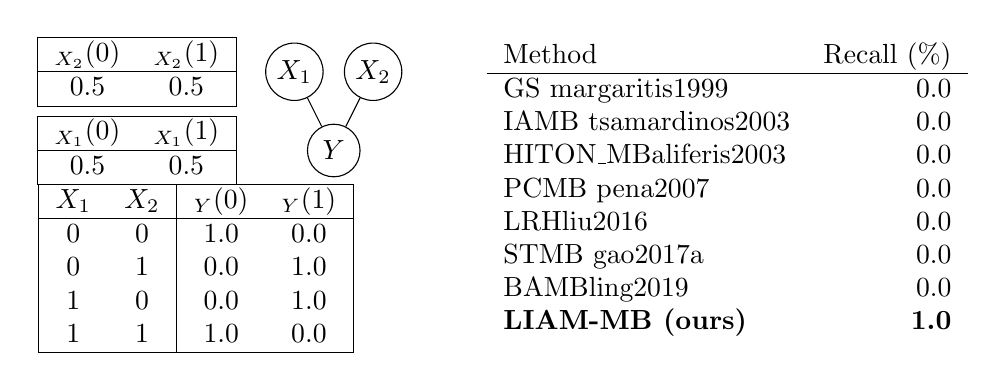
\begin{tikzpicture}
  \node[draw, circle, inner sep=2pt] (1) at (-2.5,3) {$X_{1}$};
  % \node[draw, circle, inner sep=2pt] (2) at (0,1.5) {$X_{2}$};
  \node[draw, circle, inner sep=2pt] (3) at (-1.5,3) {$X_{2}$};
  \node[draw, circle, inner sep=3pt] (y) at (-2,2) {$Y$};
  \draw (1) -- (y);
  \draw (3) -- (y);

  % \node (PrX) at (0, 2.5){
  % \begin{tabular}[t]{|cc|}
  %   \hline
  %   $\pr_{X_{i}}(0)$ & $\pr_{X_{i}}(1)$\\
  %   \hline
  %   0.5 & 0.5\\
  %   \hline
  % \end{tabular}
  % };
\node (PrX1) at (-4.5, 2){
    \begin{tabular}[t]{|cc|}
      \hline
      $\pr_{X_{1}}(0)$ & $\pr_{X_{1}}(1)$\\
      \hline
      0.5 & 0.5\\
      \hline
    \end{tabular}
};
\node (PrX2) at (-4.5, 3){
    \begin{tabular}[t]{|cc|}
      \hline
      $\pr_{X_{2}}(0)$ & $\pr_{X_{2}}(1)$\\
      \hline
      0.5 & 0.5\\
      \hline
    \end{tabular}
};


\node (PrY) at (-3.75, 0.5){
    \begin{tabular}[t]{|cc|cc|}
      \hline
      $X_{1}$ & $X_{2}$ & $\pr_{Y}(0)$ & $\pr_{Y}(1)$\\
      \hline
      0 & 0 & 1.0 & 0.0\\
      0 & 1 & 0.0 & 1.0\\
      1 & 0 & 0.0 & 1.0\\
      1 & 1 & 1.0 & 0.0\\
      \hline
    \end{tabular}
};
\node (PrY) at (3, 1.5){
    \begin{tabular}[t]{lr}
      Method & Recall (\%)\\
      \hline
      GS~\citep{margaritis1999} & 0.0\\
      IAMB~\citep{tsamardinos2003} & 0.0\\
      HITON\_MB\citep{aliferis2003} & 0.0\\
      PCMB~\citep{pena2007} & 0.0\\
      LRH\citep{liu2016} & 0.0\\
      STMB~\citep{gao2017a} & 0.0\\
      BAMB\citep{ling2019} & 0.0\\
      \textbf{LIAM-MB (ours)} & \textbf{1.0}\\
    \end{tabular}
};
\end{tikzpicture}
\caption{
  \centering
  Recovering the Markov blanket (MB) of variable $Y$ when $Y$ is
  the output of the xor boolean function between binary random variables
  $X_{1}$ and $X_{3}$. Existing approaches are unable to recover the MB
  and our approach strives to be the first step in plugging this gap.}
\end{figure}

%%%% Contributions
- pointing out gap in existing approaches
- method to prune subset lattice during exhaustive search based on g-test

%%% background
\section{Probabilistic Graphical Models and Independencies}
Consider the set of $n$ variables $\verts=\{V_{1},\ldots,V_{n}\}$ with
no other hidden or latent variables in our setting. The conditional
independencies between these variables---$\rmY \indep{} \rmX \mid \rmZ$
for disjoint variables sets $\rmY,\rmX,\rmZ\subseteq\verts$---can be
represented by either a \acrfull{dag} or an \acrfull{ug}.
% , which we denote as
% $\overrightarrow{\gr}=(\verts,\overrightarrow{\edges})$ and
% $\overline{\gr}=(\verts,\overline{\edges})$ respectively. Here
% $\overrightarrow{\edges}$ represents the set of directed edges between
% variables $\verts$ in a \acrshort{dag} while $\overline{\edges}$
% represents the undirected edges in a \acrshort{ug}.
That said, we will denote both graphs with the tuple
$\gr=(\verts,\edges)$ since we are agnostic on the type of graph used
for representing these graphical conditional independencies
$\indeps{\gr}$.
% we are only interested in the Markov blanket of a variable
% $Y\in\verts$, and are agnostic to the type of graph the Markov blanket
% arises from. As such---for the most part---we denote both types of
% graphs with the tuple $\gr=(\verts,\edges)$, where $\edges$ are the
% directed or undirected edges between the variables in $\verts$.

\paragraph{\acrfullpl{dag}} For \glspl{dag}~\citep{pearl1988}, $\edges$ consists of ordered pairs
$(V_{i},V_{j})\in\edges$ that represent the directed edges between
variables $V_{i}\rightarrow V_{j}$. The graphical conditional
independencies in a \gls{dag} are then characterised by the notion of
\emph{d-separation}~\citep{pearl1988,geiger1989}. Specifically, the
distinct variables $Y,X\in\verts$ are \emph{d-seperated} by
$\rmS\subseteq\subverts$ if all paths between $X$ and $Y$... \todo{to complete}

The vertices $Y,X\in\verts$ are
separated by $\rmS\subseteq\subverts$ in the \gls{dag} $\gr$ when 

\paragraph{\acrfullpl{ug}} On the other hand, for \glspl{ug}~\citep{lauritzen1996},

Regardless of the type of graph $\gr$ is, for disjoint subsets
$\rmX,\rmY,\rmS\subseteq\verts$, we will denote that $\rmX$ and $\rmY$
are separated in $\gr$ as,
\begin{equation}
  \label{eq:g-sep}
  \rmX \indep{\gr} \rmY \mid \rmS.
\end{equation}
Furthermore, we denote the set of conditional independencies encoded by
the graph $\gr$---i.e. the independence model of $\gr$---as,
\begin{equation}
  \label{eq:g-indeps}
  \braket{\rmX,\rmY\mid\rmS} \in \indeps{\gr}
  \iff \rmX \indep{\gr} \rmY \mid \rmS,
\end{equation}
where $\braket{\rmX,\rmY\mid\rmS}$ is known as an independence
statement~\citep{sadeghi2017}.

In addition to the graphical structure $\gr$, we also consier a joint
distribution $\pr$ over $\verts$ that might encode its own set of
conditional independencies between the variables in $\verts$,
\begin{equation}
  \label{eq:4}
  \braket{\rmX,\rmY\mid\rmS} \in \indeps{\pr}
  \iff \rmX \indep{\pr} \rmY \mid \rmS,
\end{equation}
where $\rmX \indep{\pr} \rmY \mid \rmS$ denotes $\rmX$ and
$\rmY$ are probabilistically conditionally independent given $\rmS$.

Our base assumption throughout this paper is that any
conditional independencies encoded by the graph $\gr$ implies the same
conditional independency in $\pr$---more formally known as the Global
Markov property.

\begin{assumption}[Global Markov Property]\label{def:global-markov}
  Assume we have a probabilistic graphical model $\model=(\gr,\pr)$.
  Then we say that the joint distribution $\pr$ is \emph{Markov} to the
  graph $\gr$ when for all disjoint subsets
  $\rmX,\rmY,\rmS\subseteq\verts$~\citep{hammersley1971,lauritzen2018}, 
  \begin{equation}
    \label{eq:5}
    \begin{aligned}
      &(\rmX \indep{\gr} \rmY \mid \rmS \implies
        \rmX \indep{\pr} \rmY\mid \rmS)\\
      &\iff
        \indeps{\gr} \subseteq \indeps{\pr}.
    \end{aligned}
  \end{equation}
  where
  $\braket{\rmX,\rmY\mid\rmS} \in \indeps{\pr} \iff \rmX \indep{\pr}
  \rmY \mid \rmS$. When this property holds, $\gr$ is an independency
  map, or I-map, of $\pr$.
\end{assumption}

Despite their differences, the independence models of $\gr$ and $\pr$
are both known to obey a set of axioms called the (semi-)graphoid
axioms~\citep{pearl1989}. These axioms are particully useful when
attempting to prove various theorems relating to probabilistic graphical
models.

\begin{definition}[Graphoid Axioms]\label{def:graphoid}
  For disjoint subsets $\rmX,\rmY,\rmZ,\rmW\subseteq\verts$, an
  independence model $\indeps{\cdot}$ is called a semi-graphoid if it
  obeys the following properties~\citep{dawid1979,pearl1987}:
  \begin{enumerate}
  \item Symmetry:
    $\rmX \indep{} \rmY \mid \rmZ \implies \rmY\indep{}\rmX\mid\rmZ$
  \item Decomposition:
    $\rmX \indep{} \rmY \cup \rmW \mid \rmZ \implies
    \rmX\indep{}\rmY\mid\rmZ$
  \item Weak Union:
    $\rmX\indep{}\rmY\cup\rmW\mid\rmZ \implies \rmX\indep{}\rmY \mid
    \rmW\cup\rmZ$
  \item Contraction:
    $(\rmX\indep{}\rmY \mid \rmW\cup\rmZ) \wedge
    (\rmX\indep{}\rmW\mid\rmZ)\implies \rmX\indep{}\rmY\cup\rmW\mid\rmZ$
  \end{enumerate}
  The model is called a graphoid if it obeys the folliwng additional
  property~\citep{pearl1985}:
  \begin{enumerate}[resume]
  \item Intersection:
    $(\rmX \indep{} \rmY \mid \rmZ \cup \rmW) \wedge
    (\rmX \indep{} \rmW \mid \rmZ \cup \rmY)
    \implies \rmX \indep{} \rmY \cup \rmW \mid
    \rmZ$
  \end{enumerate}
  All graph induced independence models $\indeps{\gr}$ are guranteed to
  obey all the graphoid axioms~\citep{lauritzen2018}. On the other hand,
  probabilistic independence models $\indeps{\pr}$ are only guranteed to
  obey the semi-graphoid axioms. However if the joint distribution is
  strictly positive $\pr>0$, then $\indeps{\pr}$ is guranteed to be a
  graphoid as well~\citep{pearl1988,pearl1989}.
\end{definition}

As mentioned in \Cref{sec:intro}, we are interested in learning the
graphical Markov blanket of some target variable $Y\in\verts$.
\begin{definition}[Markov Blanket and Boundary] \label{def:mb}
  For a single variable $Y\in\verts$, the Markov blanket of $Y$ in $\gr$
  is any subset $\rmM \subseteq \rmV\setminus Y$\footnote{For
    convenience we allow set operations between variables sets and
    single variables to implicitly mean the operation between the
    variable set and the atomic set containing the single variable---for
    example $\rmV \setminus Y \coloneq \rmV \setminus \{Y\}$.}
  such that every other variable in $\verts \setminus (Y \cup \rmS)$ is
  graphically separated from $Y$ by $\rmS$,
  \begin{equation}
    \label{eq:def-mb}
    Y \indep{\gr} \verts \setminus (Y \cup \rmM) \mid \rmM.
  \end{equation}
  The Markov boundary of the variable $Y$---henceforth denoted as
  $\mbs{\gr}(Y)$---is then defined as the mininal Markov blanket of
  $Y$~\citep{pearl1988}.

  An equivalent definition for the Markov blanket and boundary of $Y$ in
  $\pr$ can be made by just substituting the graph separation term in
  \Cref{eq:def-mb} for conditional independence in $\pr$.
\end{definition}
Therefore, from \Cref{def:mb}, it is more accurate to say that we wish
to learn the Markov boundary of $Y$ and not just a Markov blanket of
it. However, since colloqually the term Markov blanket is commonly used
to implicitly refer to the Markov boundary, we shall use the term Markov
blanket in such a fashion as well.

However, it is important to note that only graphs with an independence
model $\indeps{\gr}$ that satisfies the symmetry, decomoposition,
intersection, and weak union graphoid axioms in \Cref{def:graphoid} are
guranteed to have a unique Markov boundary $\mbs{\gr}(Y)$. Throughout
this paper we will assume that this is true. That said, there has been
some previous work done on addressing the case when the Markov boundary
is not unique~\citep{statnikov2013}.

-methods to learn MB
-common assumption is Faithfulness.
\begin{definition}[Faithfulness]\label{def:faith}
  Given a probabilistic graphical model $\model=(\gr, \pr)$, the graph
  $\gr$ is \emph{faithful} to the joint distribution $\pr$ if for all
  disjoint subsets $\rmX,\rmY,\rmS\subseteq\verts$~\citep{spirtes2001},
  \begin{equation}
    \label{eq:16}
    \rmX \indep{\pr} \rmY \mid \rmS
    \implies \rmX \indep{\gr} \rmY \mid \rmS
  \end{equation}
  which is also the inverse of the global Markov property in
  \Cref{def:global-markov}.
\end{definition}




%%% Faithfulness
\section{Faithfulness Violations and Existing Relaxations}
Probably the most well-known
%%% k-oder
\section{The k-Order Faithfulness Relaxation}
In this section we will introduce our generalisation of the faithfulness
assumption in \Cref{def:faith} for finding conditional dependancies that
require 

\begin{definition}[Power Sets of Limited Size]
  Let $\rmX$ be a set of elements and $k\leq |\rmX|$ be some natural
  number smaller than the cardinality of $\rmX$. Then we use the
  notation
  \begin{equation}
    \label{eq:17}
    \powereq{k}{\rmX} := \{\rmZ \subseteq \rmX : |\rmZ| = k\}
  \end{equation}
  to define the set of all the subsets of $\rmX$ with cardinality $k$
  and
  \begin{equation}
    \label{eq:18}
    \powerleq{k}{\rmX} := \{\rmZ \subseteq \rmX : |\rmZ| \leq k\}
  \end{equation}
  to denote the set of all the subsets of $\rmX$ with cardinality less
  than or equal to $k$.
\end{definition}

\begin{definition}[$k$-Order Dependence]
  For a set of random variables $\rmV$, let $Y,X\in\rmV$ and
  $\rmZ=\{Z_{1},Z_{2},\ldots,Z_{k}\}\subset\rmV$ be distinct random
  variables in $\rmV$. Let us denote the absence of any subset
  $\rmS \subseteq \rmV \setminus \{Y,X\}$ that renders $Y$ and $X$ to be
  conditionally independent given $\rmZ \cup \rmS$ as
  \begin{equation}
    \label{eq:20}
    \kassoc{\rmV}{Y,X}{\rmS}
    := \exists \rmZ \subseteq \rmV \setminus \{Y,X\} :
    Y \dep{\pr} X \mid \rmZ \cup \rmS.
  \end{equation}
  Here we say that $Y$ and $X$ are associated w.r.t. $\rmZ$.
  % Under this
  % definition, it follows that 
  % \begin{equation}
  %   \label{eq:19}
  %   \kassoc{\rmV}{Y,X}{\rmZ} \implies X \in \mb(Y)
  % \end{equation}
  % due to the absence of any probabilistic separators between $Y$ and
  % $X$.
  Of course under this definition there might be some strict subset
  $\rmZ' \subset \rmZ$ where $\kdep{\verts}{Y,X}{\rmZ'}$ still
  holds. Therefore we say $Y$ and $X$ are $|\rmZ|$-order dependent w.r.t
  $\rmZ$ only if this is not the case,
  \begin{gather}
    \begin{aligned}
      &\kdep{\rmV}{Y,X}{\rmZ}\\
      &:= \kassoc{\rmV}{Y,X}{\rmZ} \wedge
        \forall \rmZ' \subset \rmZ : \neg\, \kassoc{\rmV}{Y,X}{\rmZ'}.
    \end{aligned}
  \end{gather}
\end{definition}
difference between assoc and dep

prevents chains like
$X_{1}\rightarrow Y \rightarrow X_{2}$ to be included in this definition.

$Y\strict{k}\rmX$ results in DAGs with a collider structure, or a UG with
a clique over all the variables.
assoc
results in something
like stochastic \texttt{AND} operator.
\begin{lemma}[Finding $k$-dependance from association]
  \label{lem:k-dep-to-assoc}
  For distinct random variables $Y,X\in\rmV$ and
  $\rmX=\{X_{1},X_{2},\ldots,X_{k}\}\subset\rmV$, the following holds
  for all $\rmS \subset \rmV \setminus \rmX \cup \{Y\}$
  \begin{equation}
    \label{eq:11}
    \kassoc{k}{Y,X}{\rmS}
    \implies \exists k' \in [k] : \kdep{k'}{Y,X}{\rmS}
  \end{equation}
  where $[k]\coloneq\{i\in\mathbb{Z} : 0 \leq i \leq k\}$.
\end{lemma}
\begin{proof}[Proof by induction]
  With subsets of $\rmX$ of size $1$, $\rmZ\in\powereq{1}{\rmX}$, we
  know by definition that if $X$ and $Y$ are associated w.r.t. $\rmZ$,
  it immediately follows that $X$ and $Y$ are also $1$-dependant
  w.r.t. $\rmZ$ and vice versa,
  \begin{equation}
    \label{eq:12}
    \kassoc{\verts}{X,Y}{\rmZ}
    \iff \kdep{\verts}{X,Y}{\rmZ}.
  \end{equation}
  Now assume that $Y$ is not associated with any subsets in
  $\powerleq{k}{\rmX}$. Then we know that if $Y$ is associated with any
  subset in $\powereq{k+1}{\rmX}$, it implies a $(k+1)$-dependance
  between $X$ and $Y$. Therefore the existance of any association
  implies a potentially lower order dependance for some subset.
\end{proof}

\begin{definition}[$k$-Order Faithfulness]\label{def:k-faith}
  Given the probabilistic graphical model $\model=(\gr, \pr)$ where
  $\gr = (\verts, \edges)$, then $\gr$ is $k$-order faithful to $\pr$ if
  and only if $\forall \rmS \subseteq \verts\setminus\{Y,X\}$ whenever
  \begin{gather}
    \label{eq:k-faith-indep}
    \begin{aligned}
      &\forall \rmZ \in \power{\leq k}(\verts\setminus\{Y,X\})\:\:
        \exists \rmS' \subseteq \rmS :
      Y \indep{\pr} X \mid \rmZ \cup \rmS'\\
      &\implies
      Y \indep{\gr} X \mid \rmS,
    \end{aligned}
  \end{gather}
  More useful however is its contrapositive which states
  that $\forall \rmS \subseteq \verts\setminus\{Y,X\}$:
  \begin{gather}
    \label{eq:k-faith-1}
    \begin{aligned}
      &Y \dep{\gr} X \mid \rmS\\
      &\implies
      \exists \rmZ \in \power{\leq k}(\verts\setminus\{Y,X\}) :
      %   \forall \rmS' \subseteq \rmS :
      %   Y \dep{\pr} X \mid \rmZ \cup \rmS.
        \kassoc{\rmS}{Y,X}{\rmZ},
    \end{aligned}
    \intertext{where}
    \begin{aligned}
      \kassoc{\rmS}{Y,X}{\rmZ} \coloneq
      \forall \rmS' \subseteq \rmS : Y \dep{\pr} X \mid \rmZ \cup \rmS.
    \end{aligned}
  \end{gather}
  However, the definition in \Cref{eq:k-faith-1} allows $k$ to be larger
  than it needs to be---i.e. $k$ is not strict. Therefore, we say that
  the graph $\gr$ is \emph{strictly} $k$-order faithful to the
  distribution $\pr$ if $\forall \rmS \subseteq \verts\setminus\{Y,X\}$:
  \begin{gather}
    \label{eq:10}
    \begin{aligned}
      &Y \dep{\gr} X \mid \rmS\\
      &\implies
      \exists \rmZ \in \powereq{k}{\verts\setminus\{Y,X\}} :
      \kdep{\rmS}{Y,X}{\rmZ}
    \end{aligned}
    \intertext{where}
    \begin{aligned}
      &\kdep{\rmS}{Y,X}{\rmZ}\\
      &\coloneq
        \kassoc{\rmS}{Y,X}{\rmZ}
        \wedge
        (\forall \rmZ' \subset \rmZ :
                \neg\kassoc{\rmS}{Y,X}{\rmZ'}).
    \end{aligned}
  \end{gather}
  This implication follows directly from \Cref{lem:k-dep-to-assoc}.
% \begin{gather}
%     \begin{aligned}
%       &\forall \rmS \subseteq \subverts{YX} :
%       Y \dep{\gr} X \mid \rmS\\
%       &\implies
%       \exists \rmZ \in \power{\leq k}(\subverts{YX})\:\:
%       \forall \rmS \subseteq \subverts{YX} :
%       Y \dep{\pr} X \mid \rmZ \cup \rmS\\
%       % &\implies 
%       % \exists \rmZ \in \power{\leq k}(\subverts{YX}):
%       % \kassoc{\verts}{Y,X}{\rmZ}\\
%       % &\implies
%       % \exists \rmZ \in \power{\leq k}(\subverts{YX}):
%       % \kdep{\verts}{Y,X}{\rmZ}
%     \end{aligned}
%   \end{gather}
\end{definition}
rules out deterministic functions?

%%% Algorithm
\section{kOMB: k-order Markov Blanket}
% \begin{lemma}[Ruling out $k$-associations]
%   For distinct random variables $Y\in\rmV$ and
%   $\rmX=\{X_{1},X_{2},\ldots,X_{k}\}\subset\rmV$, the following holds
%   for all $\rmS \subset \rmV \setminus \rmX \cup \{Y\}$
%   \begin{gather}
%     \label{eq:3}
%     \begin{aligned}
%       Y\indep{}\rmX \mid \rmS
%       \implies
%       &\forall \rmZ\subseteq\rmX : Y\indep{}\rmZ \mid \rmS \cup
%         (\rmX\setminus\rmZ)\\
%       \implies
%       &Y\notassoc{\leq k}\rmX
%     \end{aligned}
%   \end{gather}
%   as a consequence of the weak union graphoid axiom.
% \end{lemma}


% \begin{lemma}[kOMB $k$-associations detection]
%   For random variables $\rmX \subset \rmV$ and
%   $Y,Z \in \rmV$, asumming $Z\in \mb(Y)$ and $k$-Adjacency Faithfulness
%   \begin{equation} 
%     \label{eq:7}
%     \begin{aligned}
%       &\bigl(\rmX \indep{} Y \mid \rmS\bigr)
%         \wedge
%         \bigl(\rmX \cup \{Z\} \dep{} Y \mid \rmS\bigr)\\
%       &\implies \exists \rmW \subseteq \rmX :
%          Y\strict{|\rmW|+1}\rmW \cup \{Z\}
%     \end{aligned}
%   \end{equation}
% \end{lemma}

\begin{lemma}[$k$-dependance implies inter-association]\label{lem:k-dep-inter}
  \begin{gather}
    \label{eq:13}
    \kdep{\rmS}{Y,X}{\rmZ}
    \implies 
    \kinter{\rmS}{Y,\rmZ \cup X}
    \intertext{where}
    \begin{aligned}
      \kinter{\rmS}{Y,\rmZ} := \forall Z\in\rmZ :
      \kassoc{\rmS}{Y,Z}{\rmZ\setminus Z}
    \end{aligned}
  \end{gather}
  by contraction
\end{lemma}
\begin{proof}
  First assume that $\kdep{\rmS}{Y,X}{\rmZ}$ which implies,
  \begin{gather}
    \begin{aligned}
      &\kdep{\rmS}{Y,X}{\rmZ}\\
      &\implies
      \forall \rmZ' \subset \rmZ \:\: \exists \rmS' \subseteq \rmS :
      Y \indep{\pr} X \mid \rmZ' \cup \rmS'
    \end{aligned}
    .\label{eq:k-dep-inter-eq2}
  \end{gather}
  Furthermore, assume that
  \begin{equation}
    \label{eq:k-dep-inter-eq1}
    \exists Z \in \rmZ \:\: \exists \rmS' \subseteq \rmS:
    Y \indep{\pr} Z \mid X \cup \rmS' \cup \rmZ \setminus Z.
  \end{equation}
  By the contraction and weak union graphoid axioms we know that for
  some $\rmS'\subseteq\rmS$,
  \begin{equation}
    \label{eq:9}
    \begin{aligned}
      &(Y \indep{\pr} Z \mid X \cup \rmS' \cup \rmZ \setminus Z)
        \wedge (Y \indep{\pr} X \mid \rmS' \cup \rmZ \setminus Z)\\
      &\implies Y \indep{\pr} \{X, Z\} \mid \rmS' \cup \rmZ \setminus Z\\
      &\implies Y \indep{\pr} X \mid \rmS' \cup \rmZ
    \end{aligned}
  \end{equation}
  However we know by definition that  
  \begin{gather}
    \label{eq:k-dep-inter-eq3}
    \kdep{\rmS}{Y,X}{\rmZ} \implies
    \forall \rmS' \subseteq \rmS : Y \dep{\pr} X \mid \rmS' \cup \rmZ,
  \end{gather}
  which causes a contradiction. Therefore, taking the negation of the
  conjunction our assumptions we get
  \begin{align*}
    &\neg \bigl(
    \kdep{\rmS}{Y,X}{\rmZ} \wedge\\
    &\qquad\exists Z \in \rmZ \:\: \exists \rmS' \subseteq \rmS: 
    Y \indep{\pr} Z \mid X \cup \rmS \cup \rmZ \setminus Z
    \bigr)\\
    &=\neg\kdep{\rmS}{Y,X}{\rmZ} \vee\\
    &\qquad\forall Z \in \rmZ \:\: \forall \rmS' \subseteq \rmS: 
    Y \dep{\pr} Z \mid X \cup \rmS \cup \rmZ \setminus Z\\
    &=\kdep{\rmS}{Y,X}{\rmZ} \implies
    \forall Z \in \rmZ :
      \kassoc{\rmS}{Y,Z}{X\cup\rmZ\setminus Z}.
  \end{align*}
  Which in addition to the implication we know to be true in
  \Cref{eq:k-dep-inter-eq3} results in
  \begin{equation}
    \label{eq:29}
    \kdep{\rmS}{Y,X}{\rmZ} \implies \kinter{\rmS}{Y, \rmZ \cup X},
  \end{equation}
  concluding our proof.
\end{proof}

\begin{lemma}[MB Subset]\label{lem:subset}
  Let $\verts' \subseteq \verts$, $X,Y \in \verts$, and $\rmZ \subseteq
  \verts \setminus (\verts' \cup \{X, Y\})$
  \begin{gather}
    \label{eq:22}
    \begin{aligned}
      \kdep{\rmS}{Y,X}{\rmZ}
      \implies \kinter{\rmS'}{Y,X\cup\rmZ}
    \end{aligned}
  \end{gather}
\end{lemma}
\begin{proof}
  For some $\rmS'\subseteq\rmS$
  \begin{align*}
    \kassoc{\rmS}{Y,X}{\rmZ}
    \iff &\forall \rmS^{*} \subseteq \rmS :
           Y \dep{\pr} X \mid \rmZ \cup \rmS^{*}\\
    \implies
         &\forall \rmS^{*} \subseteq \rmS' :
           Y \dep{\pr} X \mid \rmZ \cup \rmS^{*}\\
    \iff &\kassoc{\rmS'}{Y,X}{\rmZ}
  \end{align*}
  Using the results from \Cref{lem:k-dep-inter} and let $\rmW = X \cup
  \rmZ$, 
  \begin{align*}
    \kdep{\rmS}{Y,X}{\rmZ}
    \implies &\forall Z \in\rmZ :
               \kassoc{\rmS}{Y,Z}{X\cup\rmZ\setminus Z}\\
    \implies &\forall Z \in\rmZ :
               \kassoc{\rmS'}{Y,Z}{X\cup\rmZ\setminus Z}
  \end{align*}
  Therefore
  \begin{align*}
    \kdep{\rmS}{Y,X}{\rmZ}
    \implies\kinter{\rmS'}{Y,X\cup\rmZ}
    % &\implies
    % \kassoc{\verts'}{Y,X}{\rmZ}
    % \wedge\\
    % &\qquad
    %   \forall Z \in \rmZ : \kassoc{\verts'}{Y,Z}{X \cup \rmZ \setminus
    %   Z'}\\
    % &=\kinter{\verts'}{Y,X\cup\rmZ}
  \end{align*}
\end{proof}

needed for practical algorithm
\begin{definition}[Bounded Separator Assumption]\label{def:bound-sep}
  Let $\gr=(\verts,\edges)$, $l\in\mathbb{N}$, and assume $k$-order
  adjacency faithfulness from \Cref{def:k-faith},
  $\forall\rmS \subseteq \subverts$
  \begin{gather*}
    \begin{aligned}
      & \forall \rmZ \in \power{\leq k}(\verts\setminus\{Y,X\})\:\:
        \exists \rmS' \in \powerleq{l}{\rmS}:
        Y \indep{\pr} X \mid \rmZ \cup \rmS'\\
      &\implies
      Y \indep{\gr} X \mid \rmS,
    \end{aligned}
  \end{gather*}
  note that reversing the quantifiers here would not work, especially if $l=1$.
\begin{gather*}
  \begin{aligned}
    Y \dep{\gr} X \mid \rmS 
    &\implies
      \exists \rmZ \in \power{\leq k}(\verts\setminus\{Y,X\})\:\:
      \forall \rmS' \in \powerleq{l}{\rmS}: \\
    &\qquad\qquad Y \dep{\pr} X \mid \rmZ \cup \rmS'\\
    &\implies \exists \rmZ \in \powereq{k}{\verts\setminus\{Y,X\}}\:\:
      \forall \rmS' \in \powerleq{l}{\rmS}:\\
    &\qquad\qquad\kdep{\rmS'}{Y,X}{\rmZ}
  \end{aligned}
  \end{gather*}
  relation to global/local markov?
  Therefore, 
\end{definition}

% \begin{algorithm}
%   \caption{kOMB}
%   % \DontPrintSemicolon
%   \KwIn{$\db$, $\rmX$, $Y$, $\mb$, $\alpha$, $k$}
%   \KwOut{Output result}
%   $\verts' \gets \verts \setminus Y$\;
%   $\rmS \gets \emptyset$\tcp{CMB}
%   \While{$\exists \rmX \in [\verts']^{\leq k} :
%     Y\strict{|\rmX|}\rmX$}{
%     $\rmS \gets \rmS \cup \rmX$\;
%   }
%     \While{$\exists X \in \rmS : Y \indep{\pr} X \mid \rmS \setminus X$}{
%     $\rmS \gets \rmS \setminus X$\;
%   }
%   \Return{$\rmS$}\;
% \end{algorithm}

\begin{algorithm}
  \caption{kOMB (Pratical Implementation)}\label{alg:komb}
  % \DontPrintSemicolon
  \SetKwProg{Fn}{Function}{:}{}
  \KwIn{$\db$, $\rmX$, $Y$, $\mb$, $\alpha$, $k$, $l$}
  \KwOut{Output result}
  $\verts' \gets \verts \setminus Y$\;
  $\rmS \gets \emptyset$\tcp*[r]{Candidate Markov Blanket}
  \Repeat
  % (\tcp*[f]{While $\exists \rmX' \subseteq \rmV' \setminus \rmS : Y
  %   \strictdep{P} \rmX' \mid \rmS$})
  {$\rmX' = \emptyset$}{
    $\rmX' \gets $ find\_dep($Y$, $\emptyset$, $\rmS$, $\verts'$)\;
    $\rmS \gets \rmS \cup \rmX'$
  }
  \While{$\exists X \in \rmS : Y \indep{\pr} X \mid \rmS \setminus X$}{
    $\rmS \gets \rmS \setminus X$\;
  }
  \Return{$\rmS$}\;
\end{algorithm}


\begin{algorithm}
  \caption{Association Mining}\label{alg:assoc-mine}
  % \DontPrintSemicolon
  \SetKwProg{Fn}{Function}{:}{}
  \Fn{make\_strict($Y$, $X$, $\rmZ$, $\rmS$, $k$, $l$)}{
    \Inv{$Y \dep{} X \mid \rmX \cup \rmS$}
    % \KwOut{$\rmX'\subseteq\rmX$ s.t. $Y \dep{} X \mid \rmX' \cup \rmS$
    %   and $\forall X'\in\rmX' : Y \indep{} X \mid \rmS \cup \rmX'
    %   \setminus X'$}
    \KwOut{$X\cup\rmX'$ s.t. $\rmX'\subseteq\rmX$ and
      $\kinter{\rmS}{Y,X\cup\rmX'}$}
    \For{$Z \in \rmZ$}{
      \If{$\neg$ no\_seps($Y$, $Z$, $X\cup\rmZ
        \setminus Z$, $\rmS$, $k$, $l$)}{
        remove $Z$ from $\rmZ$\;
      }
    }
    \Return{$X\cup\rmZ$}\;
  }
  \Fn{find\_inter\_dep($Y$, $\rmX$, $\rmS$, $\rmV'$, $k$, $l$)}{
    \KwOut{$\rmX\subseteq\rmV'\setminus\rmS$
      s.t. $\kinter{\rmS}{Y,\rmX}$}
    \If{$|\rmX| > k$}{
      \Return{$\emptyset$}\;
    }
    \For{$X \in \rmV\setminus(\rmS \cup \rmX)$}{
      $\rmZ\gets$\textit{find\_cond}
      ($Y$, $X$, $\rmX$, $\rmS$, $k$, $l$)\;
      \If{$\rmZ \neq \emptyset$}{
        \tcp{$\forall \rmS'\in\powerleq{l}{\rmS} :
          Y \dep{} X \mid \rmZ \cup \rmS'$}
        \Return{make\_strict($Y$, $X$, $\rmZ$, $\rmS$, $k$, $l$)}\;
      }
    }
    \For{$X\in\rmV'\setminus(\rmS\cup\rmX)$}{
        $\rmV'\gets \rmV' \setminus X$\;
        $\rmX' \gets $ find\_inter\_dep(
        $Y$, $\rmX\cup X$, $\rmS$, $\rmV'$, $k$, $l$)\;
        \If{$\rmX' \neq \emptyset$}{
          \Return{$\rmX'$}\;
        }        
    }
    \Return{$\emptyset$}\;
  }
\end{algorithm}

\begin{algorithm}
  \caption{Practical Conditional Independence Test}\label{alg:ci-test}
  % \DontPrintSemicolon
  \SetKwProg{Fn}{Function}{:}{}
  % \KwIn{$Y$, $X$, $\rmX$, $\rmS$, $k$, $l$, $\alpha$}
  % \KwOut{is $Y \dep{} X \mid \rmX \cup \rmS$?}
  % \Inv{$\rmX \dep{} Y \mid \rmS$}
  \Fn{find\_cond($Y$, $X$, $\rmX$, $\rmS$, $k$, $l$, $\alpha$)}{
    % \KwOut{is $Y \dep{\pr} X \mid \rmX \cup \rmS$}
    \KwOut{$\exists \rmX' \in \powerleq{k-|\rmX|}{\rmS} : Y \dep{\pr} X
      \mid \rmX \cup \rmX' \cup \rmS$}
    \For{$\rmX' \in \powerleq{k'}{\rmS}$}{
      % +1 allows removing assmuption 1 from marx
      $\rmZ \gets \rmX' \cup \rmX$\;
      % $p \gets$ p-value of test $H_{0}: Y \indep{} X \mid \rmX'$\;
      \If{$Y \dep{} X \mid \rmZ$}{
        \If{no\_seps($Y$, $X$, $\rmZ$, $\rmS$, $l$, $\alpha$)}{
          \Return{$\rmZ$}\;
        }
      }
    }
    \Return{$\emptyset$}\;
  }
  \Fn{no\_seps($Y$, $X$, $\rmZ$, $\rmS$, $l$, $\alpha$)}{
    \Inv{$X \dep{} Y \mid \rmZ$}
    \KwOut{is $Y \dep{} X \mid \rmZ \cup \rmS$?}
    % max\_p $\gets 1$\;
    \For{$\rmS' \in \powerleq{l}{\rmS \setminus \rmZ}$}{
      % max\_p $\gets \min(\text{min\_p}, p)$\;
      \If{$Y \indep{} X \mid \rmZ \cup \rmS'$}{
        \Return{False}\;
      }
    }
    \Return{True}\;
  }
  
\end{algorithm}


\begin{theorem}[Correctness of \Cref{alg:ci-test}]
  \begin{equation}
    \label{eq:25}
    \exists \rmX' \in \powerleq{k}{\rmS} \:\:
    \forall \rmS' \in \powerleq{l}{\rmS \setminus \rmX'} :
    Y \dep{\pr} X \mid \rmX \cup \rmX' \cup \rmS'
  \end{equation}
\end{theorem}
% \begin{proof}
%   When called by \textit{find\_assoc}, the function \textit{not\_ci}
%   receives the subset $\rmX\in\powerleq{k}{\verts'\setminus\rmS}$ and
%   then further iterates over $\rmX'\in\powerleq{k'}{\rmS}$ where
%   $k'=\max(k-|\rmX|, 1)$. Therefore the effective search space for
%   $\rmZ := \rmX \cup \rmX'$ are the sets in $\powerleq{k+1}{\verts'}$.

%   If any of the subsets $\rmZ \in \powerleq{k+1}{\verts'}$ causes $Y$
%   and $X$ to be dependent, $Y \dep{\pr} X \mid \rmZ$, \textit{not\_ci}
%   calls \textit{no\_sep} to determine if there are any subsets in
%   $\rmS' \in \powerleq{l}{\rmS \setminus \rmZ}$ that causes $Y$ and $X$
%   to be independent, $Y \indep{\pr} X \mid \rmZ \cup \rmS'$.

%   Under the $l$-bounded separator assmuption in \Cref{def:bound-sep}, we
%   know that for some subset $\verts' \subseteq \verts\setminus\{Y,X\}$
%   \begin{align*}
%     \forall \rmS \subseteq \verts
%     &\setminus\{Y,X\} : Y \dep{\gr} X \mid \rmS\\
%     \iff
%      &\exists \rmZ \in \powerleq{k}{\verts\setminus\{Y,X\}} :
%       \ldep{\verts}{Y,X}{\rmZ}\\
%     \implies
%      &\exists \rmZ \in \powerleq{k}{\verts\setminus\{Y,X\}} :
%       \lassoc{\verts'}{Y,X}{\rmZ},
%   \end{align*}
%   which is logically equivalent to its contrapositive
%   \begin{align*}
%      &\forall\rmZ \in \powerleq{k}{\verts\setminus\{Y,X\}} \:
%       \exists \rmS' \in \powerleq{l}{\verts'} :
%        Y \indep{\pr} X \mid \rmZ \cup \rmS'\\
%      &\implies 
%        \exists \rmS^{*} \subseteq \verts
%        \setminus\{Y,X\} : Y \indep{\gr} X \mid \rmS^{*}\\
%      &\iff Y \indep{\gr} X \mid \verts \setminus \{Y,X\}
%        .
%   \end{align*}
%   Therefore, since in \Cref{alg:ci-test} $\rmS \subseteq \verts$,
%   whenever \textit{no\_seps} finds a subset of the candidate Markov
%   blanket $\rmS'\subseteq\rmS\setminus\rmZ$ that causes
%   $Y \indep{\pr} X \mid \rmZ \cup \rmS'$, we know for certain that $Y$
%   and $X$ are separated in the graph $\gr$---but the same
%   cannot be said in the reverse direction. That is to say
%   \textit{no\_seps} might not always find a separator
%   $\rmS'\subseteq\rmS$ even if $Y$ and $X$ are separated in $\gr$.

%   As a result, the function \textit{not\_ci} will only return false
%   postivies---i.e. it never indicates that $X$ and $Y$ are conditionally
%   independent when 
% \end{proof}

\begin{theorem}[Correctness of \Cref{alg:assoc-mine}]
  Given $Y$, \Cref{alg:assoc-mine}  returns
  $\rmZ=X\cup\rmX\cup\rmX'$ if
    \begin{equation*}
    \exists \rmZ \in \powerleq{k+1}{\verts\setminus Y)}
    : \linter{\rmS}{Y,\rmZ}.
  \end{equation*}
  where $(X\cup\rmX) \subseteq \verts \setminus (Y \cup \rmS)$ and
  $\rmX' \subseteq \rmS$.
\end{theorem}
\begin{proof}
  % The function \textit{find\_inter\_dep} in \Cref{alg:komb} is a
  % recursive function where for each recursive call of the function, it
  % is passed a subset of all the variables except $Y$ and $\rmS$ with
  % length less than or equal to $k$,
  % $\rmX \in \powerleq{k}{\verts' \setminus \rmS}$.

  During each function call, \textit{find\_inter\_dep} iterates through
  each varible $X$ that has not been included in $\rmX$
  yet---$X\in\verts\setminus(Y \cup \rmX \cup \rmS)$---and calls
  \textit{find\_cond} to find a set
  $\rmX' \in \powerleq{k-|\rmX|}{\rmS}$ such that
  \begin{equation*}
    \forall \rmS' \in \powerleq{l}{\rmS \setminus \rmX'} :
    Y\dep{\pr}X  \mid \rmX \cup \rmX' \cup \rmS'.
  \end{equation*}
  When such a subset $\rmX'$ is found, \textit{find\_cond} returns
  $\rmZ=X\cup\rmX'\cup\rmX$ and $\rmZ$ is then passed on to the function
  \textit{make\_strict} to remove any superfluous variables resulting in
  the set $\rmZ'\subseteq\rmZ$ such that 
  \begin{align*}
    &\forall Z \in \rmZ'\:\:
    \forall \rmS' \in \powerleq{l}{\rmS\setminus\rmZ}:
    Y \dep{\pr} Z \mid \rmZ \cup \rmS' \setminus Z\\
    &\implies \forall Z \in \rmZ' :
      \lassoc{\rmS}{Y,Z}{\rmZ\setminus Z}\\
    &\implies \linter{\rmS}{Y,X\cup\rmX\cup\rmX'}.
  \end{align*}
  Furthermore, since \textit{find\_inter\_dep} explores the
  enumeration tree of the set $\verts \setminus (Y \cup \rmS)$ up
  subsets of length $k+1$, we know that every subset
  $(X\cup\rmX)\in\powerleq{k+1}{\verts \setminus (Y \cup \rmS)}$ will be
  explored---barring any early returns. In combination with
  \textit{find\_cond} exploring the subsets $\rmX' \in
  \powerleq{k-|\rmX|}{\rmS}$, \textit{find\_inter\_dep} returns
  $\rmZ=X\cup\rmX\cup\rmX'$ if
  \begin{equation*}
    \exists \rmZ \in \powerleq{k+1}{\verts\setminus Y)}
    : \linter{\rmS}{Y,\rmZ}.
  \end{equation*}
  % Finally not that we don't explore every possible
  % $\powerleq{k}{\subverts\setminus\rmS}$ for each $X\in\verts$. But
  % this is fine... somehow
\end{proof}

\begin{theorem}[Correctness of Grow Phase in \Cref{alg:komb}]
  \begin{equation}
    \label{eq:27}
  \mbs{\gr}(Y) \subseteq \rmS 
  \end{equation}
\end{theorem}
\begin{proof}
  At each iteration of the grow phase, we obtain
  \begin{equation*}
    \rmZ : \kinter{\rmS}{Y,X\cup\rmZ}
  \end{equation*}
  since for some $\rmS\subseteq \subverts$
  \begin{align}
    &Y \dep{\gr} X \mid \verts \iff X \in \mbs{\gr}(Y)\\
    &\implies \exists \rmZ \in \powereq{k}{\subverts}:
      \kdep{\verts}{Y,X}{\rmZ}\\
    &\implies \exists \rmZ \in \powereq{k}{\subverts}:
      \kinter{\rmS}{Y,X\cup\rmZ}\\
    &\implies (X\cup\rmZ) \subseteq \rmS
  \end{align}
  where the penultimate implication follows from \Cref{lem:subset} and
  the last implication follows from line 5 of \Cref{alg:komb} where
  \method adds the subset $X\cup\rmZ$---found by the algorithm such
  that $\kinter{\rmS}{Y,X\cup\rmZ}$---into $\rmS$.
\end{proof}

%%%% Complexity
\subsection{Complexity of \method}


% \section{Lattice Incremental Association Mining for Markov Blankets
%   (LIAM-MB)}

% % \begin{figure}
% %   \centering
% %   \begin{subfigure}{0.275\linewidth}
% %     \centering
% %     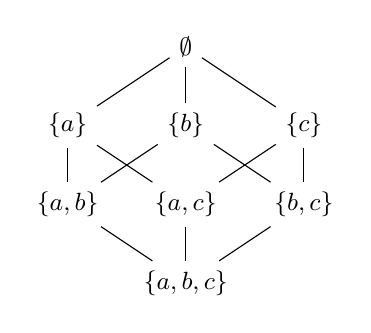
\begin{tikzpicture}[every node/.style={font=\small}]
  % Level 0
  \node (empty) at (0,0) {$\emptyset$};
  % Level 1
  \node (a) at (-1.5,-1) {$\{a\}$};
  \node (b) at (0,-1) {$\{b\}$};
  \node (c) at (1.5,-1) {$\{c\}$};
  % Level 2
  \node (ab) at (-1.5,-2) {$\{a,b\}$};
  \node (ac) at (0,-2) {$\{a,c\}$};
  \node (bc) at (1.5,-2) {$\{b,c\}$};
  % Level 3
  \node (abc) at (0,-3) {$\{a,b,c\}$};
  % Edges
  \foreach \x/\y in {
    empty/a,empty/b,empty/c,
    a/ab,a/ac,
    b/ab,b/bc,
    c/ac,c/bc,
    ab/abc,ac/abc,bc/abc}
    \draw (\x)--(\y);
\end{tikzpicture}

%%% Local Variables:
%%% mode: latex
%%% TeX-master: "../main"
%%% End:

% %     \caption{Subset Lattice}
% %     \label{fig:lattice}    
% %   \end{subfigure}
% %   \hspace{5em}
% %   \begin{subfigure}{0.325\linewidth}
% %     \centering
% %     \input{./fig/enum-tree.tex}
% %     \caption{Enumeration tree}
% %     \label{fig:tree}    
% %   \end{subfigure}
% %   \caption{Comparison between lattice and tree}
% %   \label{fig:comparison}
% % \end{figure}  
% % \begin{figure}  
% %   \begin{subfigure}{0.325\linewidth}
% %     \centering
% %     \input{./fig/enum-tree-one.tex}
% %     % \caption{$\cdf(G_{a};\df(a)) \leq \alpha$\\therefore $a$ should
% %     % be in $\mb$}
% %     \caption{\centering\\
% %       $\cdf(G_{a};\df(a)) \leq \alpha$\\ $\implies a \not\indep t
% %       \mid \mb$}
% %     \label{fig:tree}    
% %   \end{subfigure}
% %   \hfill
% %   \begin{subfigure}{0.325\linewidth}
% %     \centering
% %     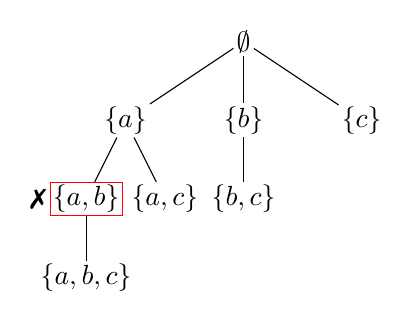
\begin{tikzpicture}[every node/.style={inner sep=1pt}]
  % Level 0
  \node (empty) at (2,0) {$\emptyset$};
  % Level 1
  \node (a) at (0.5,-1) {$\{a\}$};
  \node (b) at (2,-1) {$\{b\}$};
  \node (c) at (3.5,-1) {$\{c\}$};
  % Level 2
  \node[draw=red, label=left:{\xmark}] (ab) at (0,-2) {$\{a,b\}$};
  \node (ac) at (1,-2) {$\{a,c\}$};
  \node (bc) at (2,-2) {$\{b,c\}$};
  % % Level 3
  \node (abc) at (0,-3) {$\{a,b,c\}$};
  Edges
  \draw (empty) -- (a);
  \draw (a) -- (ab);
  \draw (ab) -- (abc);
  \draw (a) -- (ac);

  \draw (empty) -- (b);
  \draw (b) -- (bc);
  \draw (empty) -- (c);
\end{tikzpicture}

%%% Local Variables:
%%% mode: latex
%%% TeX-master: "../main"
%%% End:
% %     \caption{\centering\\
% %       $\cdf(G_{\{a,b\}};\df(\{a,b\})) > \alpha$\\
% %       $\implies \{a,b\} \indep t \mid \mb$ not rejected}
% %     \label{fig:tree}    
% %   \end{subfigure}
% %   \hfill
% %   \begin{subfigure}{0.325\linewidth}
% %     \centering
% %     \input{./fig/enum-tree-three.tex}
% %     \caption{\centering\\
% %       Prune nodes that have $\geq$ degrees of freedom than
% %       $\df(\{a,b\})$.
% %     }
% %     \label{fig:tree}    
% %   \end{subfigure}
% %   \caption{Comparison between lattice and tree}
% %   \label{fig:comparison}
% % \end{figure}

% \begin{proposition}[Maximum Testable Degrees of Freedom given a Dataset]
%   The  over all the variables of 
% \end{proposition}

% As we have discussed, our approach builds upon the two-phase approach of
% IAMB. Specifically, we want to find the variables that should be in the
% MB of $t$ that Phase \romannum{1} of IAMB did not find before the last
% pruning step.  Therefore, after the first phase IAMB, our approach will
% conduct a theorectically exhaustive search over all possible subsets
% $S \in \mathcal{P}(\rmX \setminus (\mb \cup \{t\}))$. For each subest
% $S$, our approach will test the null hypothesis
% $H_{0}(S): S \indep t \mid \mb$. The rejection of $H_{0}(S)$ implies
% that $S$---or at least a subset of $S$---belongs in the MB of $t$.  The
% total number of subsets in
% $\mathcal{P}(\rmX \setminus (\mb \cup \{t\}))$ is exponential in the
% size of $\rmR \coloneqq \rmX \setminus (\mb \cup \{t\})$. Therefore, by
% carrying out Phase \Romannum{1} of IAMB first, we can increase the size
% of $\mb$ and decrease the search space of the exhaustive search.

% % \begin{wrapfigure}{l}{0.5\linewidth}
% %   \begin{minipage}[t]{\linewidth}
% % \begin{algorithm}[H]
% %   \caption{Lattice Mining (\texttt{lattice})}
% %   % \DontPrintSemicolon
% %   \KwIn{$\db$, $\rmX$, $t$, $\mb$, $\alpha$}
% %   \KwOut{Output result}
% %   $\rmS \gets [\emptyset]$\;
% %   $\rmA \gets [\rmX]$\;
% %   $\df_{\max} \gets \infty$\; 
% %   \For{each $\rvx\in\mb$}{
% %     $S \gets \pop(\rmS)$\;
% %     $A \gets \pop(\rmA)$\;
% %     $\df_{\cur} \gets \df(\rvs)$\;
% %     \If{$|S| > 0$}{
% %       \If{$S \not\indep t \mid \mb$}{
% %         \Return{$S$}\;
% %       }
% %       \If{$1 - \cdf(G_{S\cup A}; \df(S)) > \alpha$}{
% %         $\df_{\max} \gets \df_{\cur}$\;
% %         \Comment{Pruning of supersets according to
% %           \Cref{thm:prune-superset}.}
% %         continue\; 
% %       }
% %     }
% %     \Comment{Don't explore subsets that exceed the current maximum degrees
% %       of freedom via \Cref{thm:prune}.}
% %     $A' \gets \{a \mid a\in A, \df(S \cup \{a\}) < \df_{\max}\}$\;
% %     \For{$i \in [1, |A'|]$}{
% %       $a \gets A'_{i}$\;
% %       push $S \cup \{a\}$ on to $\rmS$\;
% %       push $A'[1,\ldots,i-1]$ on to $\rmA$\;
% %     }
% %     \Return{$\emptyset$};
% %   }
% % \end{algorithm}
% % \begin{algorithm}[H]
% %   \caption{LIAM-MB}
% %   % \DontPrintSemicolon
% %   \KwIn{$\db$, $\rmX$, $t$, $\alpha$}
% %   \KwOut{Output result}
% %   $\mb \gets \texttt{forward}(\db, \rmX, t, \alpha)$\;
% %   \While{$|\rmX| > 0$}{
% %     $S \gets \texttt{lattice}(\db, \rmX, t, \mb, \alpha)$\;
% %     \If{$S==\emptyset$}{
% %       break\;
% %     }
% %     \For{$a \in S$}{
% %       Remove $a$ from $\rmX$\;
% %       Insert $a$ into $\mb$\;
% %     }
% %   }
% %   $\mb \gets \texttt{backward}(\db, \mb, t, \alpha)$\;
% %   \Return{$\mb$}\;
% % \end{algorithm}
% % \end{minipage}  
% % \end{wrapfigure}

% Since the search space is the powerset $\mathcal{P}(\rmR)$, it can be
% naturally represented as a subset lattice---see \Cref{fig:lattice} for
% an example over three variables. When traversing the subset lattice in a
% depth-first order, the resulting search order can be represented as an
% enumeration tree as seen in \Cref{fig:tree}.

% \begin{definition}[Enumeration Tree]
%   An enumeration tree $\tree$ has nodes for each subset in the powerset
%   $V(\tree)=\mathcal{P}(\rmR)$. Let $A(S)$ for some $S\in V(\tree)$ be
%   the variables in its descendants not in $S$. Let $S_{i}$ be the $i$-th
%   node visited during a depth-wise traversal of the corresponding
%   lattice. Then by definition:
%   \begin{equation}
%     \label{eq:set-enum}
%     S_{i}\cup A(S_{i}) \supseteq S_{j}\cup A(S_{j})
%   \end{equation}
%   where $j > i$.
% \end{definition}

% The property in \Cref{eq:set-enum} will allow us to prune chunks of the
% search space based on properties of $S_{i}$. Specifically we desire a
% way to determine at subset $S_{i}$ which proceeding subsets
% $j>i : S_{j}$ will not be capable of rejecting the conditional
% independence test.

% \begin{theorem}[Pruning based on maximum degrees of freedom]
%   \label{thm:prune}
%   At some node in the enumeration tree $(S_{i}, A_{i})$, if
%   \begin{equation}
%     \label{eq:df-max-reject}
%     1 - F(G_{S_{i}\cup A_{i}}; \df(S_{i})) > \alpha
%   \end{equation}
%   then for every subsequent node in the enumeration tree $S_{j}, j > i$
%   \begin{equation}
%     \label{eq:df-max-reject}
%     \df(S_{j}) \geq \df(S_{i}) \implies
%     1 - F(G_{S_{j}\cup A_{i}}; \df(S_{j})) > \alpha
%   \end{equation}
% \end{theorem}
% \begin{proof}
%   First recall from the definition of enumeration trees that
%   \begin{equation*}
%     S_{i} \cup A(S_{i}) \supseteq S_{j} \cup A(S_{j})
%   \end{equation*}
%   for all $i \geq j$. Therefore, by using \Cref{thm:chi2-ineq,thm:dpi}
%   with the assumption that $\df(S_{j}) \geq \df(S_{i})$,
%   we can establish the following inequality:
%   \begin{gather*}
%     F(G_{S_{i}\cup A(S_{i})}; \df(S_{i}))
%     \underset{\text{\Cref{thm:dpi}}}{\geq}
%     F(G_{S_{j}\cup A(S_{j})}; \df(S_{i}))
%     \underset{\text{\Cref{thm:chi2-ineq}}}{\geq}
%     F(G_{S_{j}\cup A(S_{j})}; \df(S_{j}))\\
%     \implies 1 - F(G_{S_{i}\cup A(S_{i})}; \df(S_{i}))
%     \leq 1 - F(G_{S_{j}\cup A(S_{j})}; \df(S_{j}))
%   \end{gather*}
%   Therefore the following holds
%   \begin{align*}
%     \alpha < 1 - \cdf(G_{S_{i}\cup A(S_{i})}; \df(S_{i}))
%     \implies 
%     \alpha <  1 - \cdf(G_{S_{j}\cup A(S_{j})}; \df(S_{j}))
%   \end{align*}
%   whenever $\df(S_{j}) \geq \df(S_{i})$.
% \end{proof}
% \begin{corollary}[Pruning Supersets]
%   \label{thm:prune-superset}
%   At some node in the enumeration tree $S_{i}$, if
%   \begin{equation}
%     \label{eq:max-reject}
%     1 - F(G_{S_{i}\cup A(S_{i})}; \df(S_{i})) > \alpha
%   \end{equation}
%   where $\alpha$ is some prescribed significance level, then it follows
%   directly from \Cref{thm:prune} that
%   \begin{equation}
%     \label{eq:max-pruned}
%     \forall S' \supseteq S : 1 - \cdf(G_{S'}; \df(S')) > \alpha
%   \end{equation}
%   since $S' \supseteq S \implies \df(S') \geq \df(S)$.
%   % therefore, when \Cref{eq:max-reject} is true, no superset of $S$ can
%   % have their conditional independence hypothesis be
%   % rejected. Consequently, we cannont definitively accept the hypothesis
%   % that any superset of $S$ is in the MB of $t$.
% \end{corollary}

% This implies that at $S_{i}$, we can prune entire branch.

% - conjecture same result as IAMB
% - Complexity?
% - 

%%% Experiments
\section{Experiments}\label{sec:exp}
Throughout this section we will compare our approach against existing
methods for Markov blanket discovery. Specifically we will compare
against the following nine Markov blanket discovery mehtods:
\begin{itemize}
\item GS~\citep{margaritis1999}. 
\item IAMB~\citep{tsamardinos2003}.
\item HITON~\citep{aliferis2003}.
\item PCMB~\citep{pena2007}.
\item LRH~\citep{liu2016}.
\item STMB~\citep{gao2017a}.
\item BAMB~\citep{ling2019}.
\end{itemize}
For our experiments, we will use the implementation of these methods
found in the \texttt{pyCausalFS} python library~\citep{yu2020a} with a
significance level of $0.01$ for any statistical tests. When comparing
the methods above we will use the metric \emph{recall}---the percentage
of the variables in the true Markov blanket recovered by the Markov
blanket discovery method.


\subsection{Experiments with Synthetic Bayesian Networks}
\begin{figure}
  \centering
  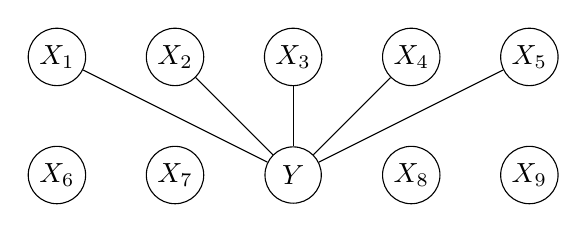
\begin{tikzpicture}[every node/.style={draw, circle, inner sep=2pt}]
  \node[inner sep=3.5pt] (y) at (0,0) {$Y$};
  \node (x1) at (-3,1.5) {$X_{1}$};
  \node (x2) at (-1.5,1.5) {$X_{2}$};
  \node (x3) at (0,1.5) {$X_{3}$};
  \node (x4) at (1.5,1.5) {$X_{4}$};
  \node (x5) at (3,1.5) {$X_{5}$};

  \node (x6) at (-3,0) {$X_{6}$};
  \node (x7) at (-1.5,0) {$X_{7}$};
  \node (x8) at (1.5,0) {$X_{8}$};
  \node (x9) at (3,0) {$X_{9}$};

  \draw (x1) -- (y);
  \draw (x2) -- (y);
  \draw (x3) -- (y);
  \draw (x4) -- (y);
  \draw (x5) -- (y);
  \end{tikzpicture}
\end{figure}
In order to empirically determine situations where non-exhaustive
heuristic approaches might have difficulty discovering the Markov
blanket of a variable, in this section we will keep it simple focus on
discovering the Markov blanket of variables that are the output of some
Boolean function. Specifically, we will use following Boolean functions:
\begin{description}[align=right,labelwidth=7em]
\item[parity:]     
  $f(X_{1},\ldots,X_{5}) = (\sum_{i=1}^{5}X_{i}) \mod 2$
\item[prime:]      
  $f(X_{1},\ldots,X_{5}) = \bigl[(\sum_{i=1}^{5}X_{i}) \text{ is prime}\bigr]$
\item[exactly-$k$:] 
  $f(X_{1},\ldots,X_{5}; k) = \bigl[(\sum_{i=1}^{5}X_{i}) = k\bigr]$
\item[and:]        
  $f(X_{1},\ldots,X_{5}) = \bigl[(\sum_{i=1}^{5}X_{i}) = 5\bigr]$
\item[or:]         
  $f(X_{1},\ldots,X_{5}) = \bigl[(\sum_{i=1}^{5}X_{i}) \geq 1\bigr]$
\end{description}
We then construct a Bayesian network for each 


% \begin{tabular}{lrrrrrrrrrr}
\toprule
{} & \multicolumn{2}{c}{and} & \multicolumn{2}{c}{ex-1} & \multicolumn{2}{c}{ex-2} & \multicolumn{2}{c}{or} & \multicolumn{2}{c}{parity} \\
method & mean & std & mean & std & mean & std & mean & std & mean & std \\
\midrule
BAMB & 0.347500 & 0.341180 & 0.215000 & 0.274142 & 0.217500 & 0.296031 & 0.327500 & 0.317835 & 0.025000 & 0.110361 \\
GSMB & 0.410000 & 0.404969 & 0.312500 & 0.418904 & 0.287500 & 0.406478 & 0.365000 & 0.373857 & 0.025000 & 0.110361 \\
HITON\_MB & 0.347500 & 0.341180 & 0.215000 & 0.274142 & 0.217500 & 0.296031 & 0.327500 & 0.317835 & 0.025000 & 0.110361 \\
IAMB & 0.410000 & 0.404969 & 0.312500 & 0.418904 & 0.287500 & 0.406478 & 0.365000 & 0.373857 & 0.025000 & 0.110361 \\
LRH & 0.410000 & 0.404969 & 0.312500 & 0.418904 & 0.287500 & 0.406478 & 0.365000 & 0.373857 & 0.025000 & 0.110361 \\
MMMB & 0.347500 & 0.341180 & 0.215000 & 0.274142 & 0.217500 & 0.296031 & 0.327500 & 0.317835 & 0.025000 & 0.110361 \\
PCMB & 0.327500 & 0.337401 & 0.215000 & 0.274142 & 0.205000 & 0.294348 & 0.315000 & 0.320696 & 0.025000 & 0.110361 \\
STMB & 0.400000 & 0.392232 & 0.277500 & 0.363380 & 0.267500 & 0.373746 & 0.350000 & 0.350823 & 0.025000 & 0.110361 \\
kOMB-0-1 & 0.410000 & 0.404969 & 0.282500 & 0.372027 & 0.267500 & 0.373746 & 0.350000 & 0.350823 & 0.025000 & 0.110361 \\
kOMB-0-2 & 0.410000 & 0.404969 & 0.282500 & 0.372027 & 0.267500 & 0.373746 & 0.350000 & 0.350823 & 0.025000 & 0.110361 \\
kOMB-0-3 & 0.410000 & 0.404969 & 0.282500 & 0.372027 & 0.267500 & 0.373746 & 0.350000 & 0.350823 & 0.025000 & 0.110361 \\
kOMB-1-1 & 0.617500 & 0.374089 & 0.675000 & 0.474342 & 0.675000 & 0.474342 & 0.560000 & 0.434889 & 0.050000 & 0.220721 \\
kOMB-1-2 & 0.617500 & 0.374089 & 0.675000 & 0.474342 & 0.675000 & 0.474342 & 0.560000 & 0.434889 & 0.050000 & 0.220721 \\
kOMB-1-3 & 0.617500 & 0.374089 & 0.675000 & 0.474342 & 0.675000 & 0.474342 & 0.560000 & 0.434889 & 0.050000 & 0.220721 \\
kOMB-2-1 & 0.617500 & 0.374089 & 1.000000 & 0.000000 & 1.000000 & 0.000000 & 0.710000 & 0.384174 & 1.000000 & 0.000000 \\
kOMB-2-2 & 0.617500 & 0.374089 & 1.000000 & 0.000000 & 1.000000 & 0.000000 & 0.710000 & 0.384174 & 1.000000 & 0.000000 \\
kOMB-2-3 & 0.617500 & 0.374089 & 1.000000 & 0.000000 & 1.000000 & 0.000000 & 0.710000 & 0.384174 & 1.000000 & 0.000000 \\
\bottomrule
\end{tabular}


\begin{table*}
  \centering
  % \begin{table}[t]
% \centering
% \scriptsize
\setlength{\tabcolsep}{5pt}
% \renewcommand{\arraystretch}{1.05}
\begin{tabular}{lccccc}
\toprule
Method & and & ex-1 & ex-2 & or & parity \\
\midrule

BAMB
& 0.348 & 0.215 & 0.218 & 0.328 & 0.025 \\
& {\scriptsize $\pm$0.341} & {\scriptsize $\pm$0.274} & {\scriptsize $\pm$0.296} & {\scriptsize $\pm$0.318} & {\scriptsize $\pm$0.110} \\

GSMB
& 0.410 & 0.313 & 0.288 & 0.365 & 0.025 \\
& {\scriptsize $\pm$0.405} & {\scriptsize $\pm$0.419} & {\scriptsize $\pm$0.407} & {\scriptsize $\pm$0.374} & {\scriptsize $\pm$0.110} \\

HITON\_MB
& 0.348 & 0.215 & 0.218 & 0.328 & 0.025 \\
& {\scriptsize $\pm$0.341} & {\scriptsize $\pm$0.274} & {\scriptsize $\pm$0.296} & {\scriptsize $\pm$0.318} & {\scriptsize $\pm$0.110} \\

IAMB
& 0.410 & 0.313 & 0.288 & 0.365 & 0.025 \\
& {\scriptsize $\pm$0.405} & {\scriptsize $\pm$0.419} & {\scriptsize $\pm$0.407} & {\scriptsize $\pm$0.374} & {\scriptsize $\pm$0.110} \\

LRH
& 0.410 & 0.313 & 0.288 & 0.365 & 0.025 \\
& {\scriptsize $\pm$0.405} & {\scriptsize $\pm$0.419} & {\scriptsize $\pm$0.407} & {\scriptsize $\pm$0.374} & {\scriptsize $\pm$0.110} \\

MMMB
& 0.348 & 0.215 & 0.218 & 0.328 & 0.025 \\
& {\scriptsize $\pm$0.341} & {\scriptsize $\pm$0.274} & {\scriptsize $\pm$0.296} & {\scriptsize $\pm$0.318} & {\scriptsize $\pm$0.110} \\

PCMB
& 0.328 & 0.215 & 0.205 & 0.315 & 0.025 \\
& {\scriptsize $\pm$0.337} & {\scriptsize $\pm$0.274} & {\scriptsize $\pm$0.294} & {\scriptsize $\pm$0.321} & {\scriptsize $\pm$0.110} \\

STMB
& 0.400 & 0.278 & 0.268 & 0.350 & 0.025 \\
& {\scriptsize $\pm$0.392} & {\scriptsize $\pm$0.363} & {\scriptsize $\pm$0.374} & {\scriptsize $\pm$0.351} & {\scriptsize $\pm$0.110} \\

kOMB-1-1
& 0.595 & 0.538 & 0.538 & 0.460 & 0.000 \\
& {\scriptsize $\pm$0.361} & {\scriptsize $\pm$0.402} & {\scriptsize $\pm$0.411} & {\scriptsize $\pm$0.364} & {\scriptsize $\pm$0.000} \\

kOMB-1-2
& \textbf{0.618} & 0.775 & 0.775 & 0.610 & 0.050 \\
& {\scriptsize $\pm$0.374} & {\scriptsize $\pm$0.423} & {\scriptsize $\pm$0.423} & {\scriptsize $\pm$0.425} & {\scriptsize $\pm$0.221} \\

kOMB-2-1
& \textbf{0.618} & \textbf{1.000} & \textbf{1.000} & \textbf{0.710} & \textbf{1.000} \\
& {\scriptsize $\pm$0.374} & {\scriptsize $\pm$0.000} & {\scriptsize $\pm$0.000} & {\scriptsize $\pm$0.384} & {\scriptsize $\pm$0.000} \\

kOMB-2-2
& \textbf{0.618} & \textbf{1.000} & \textbf{1.000} & \textbf{0.710} & \textbf{1.000} \\
& {\scriptsize $\pm$0.374} & {\scriptsize $\pm$0.000} & {\scriptsize $\pm$0.000} & {\scriptsize $\pm$0.384} & {\scriptsize $\pm$0.000} \\

\bottomrule
\end{tabular}
% \caption{Mean performance (regular font) and standard deviation (script size) across synthetic datasets. Best mean per dataset in bold.}
% \end{table}
%%% Local Variables:
%%% mode: latex
%%% TeX-master: "../main"
%%% End:

  \caption{Synthetic Results}
  \label{tab:syn}
\end{table*}

\subsection{Experiments with Benchmark Bayesian Networks}


%%% Post matter
% \subsubsection*{Author Contributions}
% If you'd like to, you may include a section for author contributions
% as is done in many journals. This is optional and at the discretion of
% the authors.

% \subsubsection*{Acknowledgments}
% Use unnumbered third level headings for the acknowledgments. All
% acknowledgments, including those to funding agencies, go at the end of
% the paper.



\bibliography{ref}
\bibliographystyle{iclr2026_conference}

\appendix
\section{Appendix}
You may include other additional sections here.
\subsection{G-Test}
The G-test is a statistical test that seeks to reject the hypothesis
that a set of observed discrete data follows some assumed
distribution. A common use for the G-test is to test if the dimensions
in some multidimensional data are independent. Conducting this test
first involves computing the G-statistic,
\begin{equation}
  \label{eq:g-stat}
  G = 2 \sum_{i} O_{i}\cdot \ln\Biggl(\frac{O_{i}}{E_{i}}\Biggr),
\end{equation}
where $O_{i}\geq 0$ are the observed counts in the cells and $E_{i} > 0$
are the expected counts under the distribution assumed in the null
hypothesis.

In this paper, we are specifically interested in using the G-test to
test the null hypothesis that some subset $\rmS$ of the variables
$\rmS\subset\rmX \setminus (\{\rvt\} \cup \mb)$ is conditionally
independent to the variable $\rvt$ given the a candidate Markov blanket
$\mb$,
\begin{equation*}
  H_{0}(\rmS): \rmS \indep \rvt \mid \mb.
\end{equation*}
The G-statistic for testing this hypothesis is
then~\citep{tsamardinos2006}
\begin{align*}
  G(\rmS)
  &= 2 \sum_{\rvx_{\rvs},\rvx_{t},\rvx_{\rvc}}
    O(\rvx_{\rvs},\rvx_{t},\rvx_{\rvc})\cdot
    \ln\Biggl(
    \frac{P(\rvx_{\rvs},\rvx_{t}\mid\rvx_{\rvc}) P(\rvx_{\rvc})}
    {P(\rvx_{\rvs}\mid\rvx_{\rvc})P(\rvx_{t}\mid\rvx_{\rvc})
    P(\rvx_{\rvc})}\Biggr)\\
  &= 2 \sum_{\rvx_{\rvs},\rvx_{t},\rvx_{\rvc}}
    O(\rvx_{\rvs},\rvx_{t},\rvx_{\rvc})\cdot
    \ln\Biggl(
    \frac{O(\rvx_{\rvs},\rvx_{t},\rvx_{\rvc}) O(\rvx_{\rvc})}
    {O(\rvx_{\rvs},\rvx_{\rvc})O(\rvx_{t},\rvx_{\rvc})}\Biggr).
\end{align*}
Under the null hypothesis, the distribution of this statistic $G(\rmS)$
is then approximately $\chi^{2}(\df(\rmS))$ distributed
where~\citep{tsamardinos2006}
\begin{align*}
  \df(\rmS) &= (|\rvt|-1) \cdot
              \Biggl(\prod_{\rvs\in\rmS}|\rvs| - 1\Biggr) \cdot
              \Biggl(\prod_{\rvc\in\mb}|\rvc|\Biggr)
\end{align*}
is the degrees of freedomn in the statistical test. 



\end{document}

%%% Local Variables:
%%% mode: latex
%%% TeX-master: t
%%% End:
